%%%%%     $Id: simple_fm_receiver.tex,v 1.1 2005-01-25 04:46:05 arif_endro Exp $
%%%%%%%%%%%%%%%%%%%%%%%%%%%%%%%%%%%%%%%%%%%%%%%%%%%%%%%%%%%%%%%%%%%%%%%%%%%%%%%%%%%%%%%%%%%%%%%%%
%%%%%     Title      : Simple FM Receiver DOCS
%%%%%     Project    : FM Receiver
%%%%%%%%%%%%%%%%%%%%%%%%%%%%%%%%%%%%%%%%%%%%%%%%%%%%%%%%%%%%%%%%%%%%%%%%%%%%%%%%%%%%%%%%%%%%%%%%%
%%%%%     Author     : Arif E. Nugroho
%%%%%  
%%%%%%%%%%%%%%%%%%%%%%%%%%%%%%%%%%%%%%%%%%%%%%%%%%%%%%%%%%%%%%%%%%%%%%%%%%%%%%%%%%%%%%%%%%%%%%%%%
%%%%%    Description : Simple FM Receiver documentations file
%%%%%%%%%%%%%%%%%%%%%%%%%%%%%%%%%%%%%%%%%%%%%%%%%%%%%%%%%%%%%%%%%%%%%%%%%%%%%%%%%%%%%%%%%%%%%%%%%
%%%%%    Copyright (c) 2005 Arif E. Nugroho
%%%%%    This VHDL design file is an open design; you can redistribute it and/or
%%%%%    modify it and/or implement it after contacting the author
%%%%%%%%%%%%%%%%%%%%%%%%%%%%%%%%%%%%%%%%%%%%%%%%%%%%%%%%%%%%%%%%%%%%%%%%%%%%%%%%%%%%%%%%%%%%%%%%%

\documentclass[a4paper,10pt]{article}
\usepackage[dvips]{graphics}
\usepackage[english]{babel}
\usepackage{doublespace}
\usepackage{epsf}
\usepackage{fancybox}
\usepackage{fancyheadings}
\usepackage{float}
\usepackage{graphicx}
\usepackage{here}
\usepackage{rotate}
\usepackage{isolatin1}
\usepackage{palatino}
\usepackage{picinpar}
\usepackage{psfig}
\usepackage{rotate}
\usepackage{subfigure}
\usepackage{sverb}
\usepackage{t1enc}
\usepackage{wrapfig}

\setlength{\topmargin}     {0cm}
\setlength{\headheight}    {1cm}
\setlength{\textheight}    {21cm}
\setlength{\textwidth}     {16cm}
\setlength{\oddsidemargin} {0cm}
\setlength{\evensidemargin}{0cm}
\setlength{\columnsep}     {0.125in}
\setlength{\columnseprule} {0.5pt}
\setlength{\footskip}      {1cm}
\renewcommand{\headrulewidth}{0.4pt}
\renewcommand{\footrulewidth}{0.4pt}
\setstretch{1}

\newlength{\verbatimbox}
\settowidth{\verbatimbox}{\scriptsize\tt
xxxxxxxxxxxxxxxxxxxxxxxxxxxxxxxxxxxxxxxxxxxxxxxxxxxxxxxxxxxxxxxxxxxxxxxxxxxxxxxx
}

\newlength{\verbatimboxhalf}
\settowidth{\verbatimboxhalf}{\scriptsize\tt
xxxxxxxxxxxxxxxxxxxxxxxxxxxxxxxxxxxxxxxx
}

\newenvironment{sourcelisting}
   {\VerbatimEnvironment\par\noindent\scriptsize
    \begin{Sbox}\begin{minipage}{\verbatimbox}\begin{Verbatim}}%
   {\end{Verbatim}\end{minipage}\end{Sbox}
    \setlength{\fboxsep}{3mm}\center
    \shadowbox{\TheSbox}\normalsize\par\noindent}

\newenvironment{sourcelistingtiny}
   {\VerbatimEnvironment\par\noindent\tiny
    \begin{Sbox}\begin{minipage}{\verbatimboxhalf}\begin{Verbatim}}%
   {\end{Verbatim}\end{minipage}\end{Sbox}
    \setlength{\fboxsep}{3mm}\center
    \shadowbox{\TheSbox}\normalsize\par\noindent}

\newenvironment{commandline}
   {\VerbatimEnvironment\par\vspace*{2mm}\noindent\footnotesize
    \begin{Sbox}\begin{minipage}{\verbatimbox}\begin{Verbatim}}%
   {\end{Verbatim}\end{minipage}\end{Sbox}\setlength{\shadowsize}{2pt}%
    \shadowbox{\TheSbox}\normalsize\par\noindent}

\renewcommand {\thefigure}{\arabic{section}-\arabic{figure}}

\pagestyle{fancy}
\chead{}
\lhead{\Large \bfseries \texttt{Simple FM Receiver}}
\rhead{\bfseries \texttt{\leftmark} \hspace{0.5cm}}
\rfoot{\bfseries \texttt{Arif E. Nugroho}}
\cfoot{www.opencores.org}
\lfoot{\bfseries \texttt{\thepage}}
\newcommand { \ssection } [1] { %
    {\section [#1] {\centering \sc \bf \\ #1 } } }
\begin{document}
\pagenumbering{roman}
\thispagestyle{empty}
\begin{center}
\Huge \textbf {\textit{Simple FM Receiver}}\\
\vspace{3.0cm}
%\large \textbf {\texttt{Arif E. Nugroho \\<arif\_endro@yahoo.com>}}
\large \textbf {\texttt{Arif E. Nugroho \\<arif\_endro@opencores.org>}}
\vspace{3.0cm}
\end{center}

\begin{figure}[H]
\center
\includegraphics[width=7.5cm,height=7.5cm]{fm_cores.eps}
\end{figure}

\vspace{0.50cm}
\begin{tabular}{p{3.0cm}p{10cm}}
		& VLSI Research Group ITB\\
		& LabTek VIII Institut Teknologi Bandung\\
		& Jl. Ganesha 10 Bandung 40141 West Java Indonesia\\
\end{tabular}


\vspace{1.00cm}
\begin{center}

\Large \textbf{\texttt{2005}}
\end{center}

\newpage

\tableofcontents
\newpage

\listoffigures
\newpage
\pagenumbering{arabic}
\setcounter{figure}{0}

\section{Circuit Block}
   Simple FM Receiver is based on PLL operation to capture FM input
   data. The design architecture is like ordinary PLL using basic component
   like phase detector, vco (realize using an nco), loop filter, and other
   supporting component.
\begin{figure}[H]
\center
\includegraphics[width=15cm,height=12cm]{fm_receiver.eps}
\caption {Architecture Schematics}
\end{figure}
   This design is based on example circuit in 
   \textbf{Mr. Wada} homepage with some modification.

\setcounter{figure}{0}
\section{Circuit Explanation}
\subsection{Core Component}
   \begin{itemize}
   \item \textbf{fm}\\
   		It's the main component, it's purpose is to connect
                many other component to form an PLL. It's function is to 
		demodulate the FM data.

\begin{figure}[H]
\center
\includegraphics[width=10.0cm,height=5.0cm]{fm.eps}
\caption {FM core component}
\end{figure}

   \end{itemize}
\subsection{Main Component}
   \begin{itemize}
   \item \textbf{nco}\\ 
   		The NCO functions it's like VCO in analog PLL. 
   		This NCO works like variable binary up-counter that controlled 
		by input. Because its controlled by input then it's output
		frequency is change along with it's input value.

\begin{figure}[H]
\center
\includegraphics[width=10.0cm,height=5.0cm]{nco.eps}
\caption {NCO block diagram}
\end{figure}

   \item \textbf{phase\_detector}\\ 
   		It's functions is to detect the phase
                different between input signal and signal from nco. This
		component is operate by multiplying input signal and output NCO.

\begin{figure}[H]
\center
\includegraphics[width=10.0cm,height=5.0cm]{phase_detector.eps}
\caption {Phase detector block diagram}
\end{figure}

   \item \textbf{loop\_filter}\\
   		The filter that exists in the PLL loop. It's mathematical
		functions look like this. 
		\begin{displaymath}
		Y(z) = X(z) \frac{z^{-1}}{1-(1-\frac{1}{16})z^{-1}}
		\end{displaymath}

\begin{figure}[H]
\center
\includegraphics[width=10.0cm,height=5.0cm]{loop_filter.eps}
\caption {Loop filter block diagram}
\end{figure}

   \item \textbf{fir}\\ 
   		This is the Low Pass filter type FIR. 
   		Realization of filter using direct FIR Transform 16 tap.
		\begin{displaymath}
		Y(z) = X(z) \frac{1}{16}\sum_{i=0}^{15}z^{-i}
		\end{displaymath}
   \end{itemize}
\subsection{Basic Component}
   \begin{itemize}
   \item \textbf{adder}\\ 
   		Many customized adder have been used on this design.
   		This adder is used for many aritmetic operation, special
		purpose adder were used for aritmetics operation in 
		2's complement or unsigned number.
   \item \textbf{subtractor}\\ 
   		The subtractor that used on the loop filter,
   		we realize the loop filter constant multiplier e.g. (15/16) by
		(1 - 1/16) so we need a substractor to do this task. Actually we
		implement the substractor by using ordinary adder, but the 
		augend is 2's complement of subtractor.

\begin{sourcelisting}
                - X = 2's (X)       (negatif value is equal to 2's of it's value)
              X - Y = X + 2's (Y)
\end{sourcelisting}

   \item \textbf{multiplier}\\ 
   		Multiplier is used on the phase detector to
   		multiply input signal and signal nco to get the phase different.
		This multiplier is implemented using simple addition of two
		operand,  this multiplier need 8 stage of addition to perform
		operation on 8 bit input operand. This multiplier is the 
		slowest component in this design, because this operations 
		takes 8 stages of additions to complete single multiplications.
\begin{sourcelisting}
operand0          = XXXX_XXXX
operand1          = XXXX_XXXX
_____________________________
...
...       -> 8 stage addition
...
_____________________________
result = XXXX_XXXX__XXXX_XXXX
         ^^^^^^^^^--> 8 bit output
\end{sourcelisting}
   \item \textbf{full adder}\\ 
   		The very basic component that build all module.
		This component is implemented using this relations.\\
\begin{sourcelisting}
sum          <=  ((addend xor augend) xor carry_in);
carry        <=  ((addend xor augend) or  (carry_in and (addend or augend)));
\end{sourcelisting}
   \end{itemize}

\setcounter{figure}{0}
\newpage
\section{Information}
%\subsection{Cover Image}
%Figure in the cover of this docs  is the looks of wafer layout of simple\_fm\_receiver
%core design (e.g. only the core not includes ROM, NCO, Phase detector, FIR), 
%this figure is generated using \texttt{\textbf{Alliance}} tools.

%\subsection{HDL Source}
%The source codes is available at:
%\begin{itemize}
%\item \textbf{\texttt{WWW}}\\
%      The HDL source is available using World Wide Web access located at:\\
%      \texttt{http://students.ee.itb.ac.id/\~\ arif\_endro/simple\_fm\_receiver/}
%\item \textbf{\texttt{CVS}}\\
%      The HDL development source is available using cvs server:\\
%      \texttt{cvs -z3 -d :pserver:anonymous@cvs.opencores.org:/cvsroot/anonymous}\\
%      the password for anonymous user is empty (e.g. blank password). and 
%      the cvs modules is: \\\textbf{simple\_fm\_receiver}
%\end{itemize}

\subsection{Warranty}
\begin{center}
		\textbf	     {\texttt{NO WARRANTY}}\\
\end{center}
\scriptsize
\textbf{\textrm{
THIS SOFTWARE IS PROVIDED BY THE AUTHOR ``AS IS'' AND ANY EXPRESS OR
IMPLIED WARRANTIES, INCLUDING, BUT NOT LIMITED TO, THE IMPLIED WARRANTIES
OF MERCHANTABILITY AND FITNESS FOR A PARTICULAR PURPOSE ARE DISCLAIMED.
IN NO EVENT SHALL THE AUTHOR BE LIABLE FOR ANY DIRECT, INDIRECT,
INCIDENTAL, SPECIAL, EXEMPLARY, OR CONSEQUENTIAL DAMAGES (INCLUDING, BUT
NOT LIMITED TO, PROCUREMENT OF SUBSTITUTE GOODS OR SERVICES; LOSS OF USE,
DATA, OR PROFITS; OR BUSINESS INTERRUPTION) HOWEVER CAUSED AND ON ANY
THEORY OF LIABILITY, WHETHER IN CONTRACT, STRICT LIABILITY, OR TORT
(INCLUDING NEGLIGENCE OR OTHERWISE) ARISING IN ANY WAY OUT OF THE USE OF
THIS SOFTWARE, EVEN IF ADVISED OF THE POSSIBILITY OF SUCH DAMAGE.}}
\normalsize

\subsection{TOOLS}
\begin{itemize}
\item \textbf{\texttt{ALLIANCE CAD SYSTEM}} developed by \textbf{\texttt{ASIM}}
      team at \copyright \textbf{\texttt{LIP6}}/Universit\'{e} Pierre et
      Marie Curie,
      \texttt{http://asim.lip6.fr/recherche/alliance} 
      - \textbf{\textit{The primary VHDL Analyser for Synthesize}}
\item \textbf{\texttt{ModelSim 6.0}} - \textbf{\textit{The Simulator}}
\item \textbf{\texttt{ISE Xilinx 6.3i}} - \textbf{\textit{The Synthesizer}}
\item \textbf{\texttt{FPGA Xilinx XC2V2000-6-FF896}} - \textbf{\textit{The Implementor}}
\item \textbf{\texttt{VIM - Vi IMproved}} 
      - \textbf{\textit{The Editor}}
\item \LaTeX - \textbf{\textit{The Typesetter}}
\end{itemize}

\begin{thebibliography}{1}
%\bibitem{Navabi} Zainalabedin Navabi,
%        \textbf{\textit{ VHDL Analysis and Modeling of Digital Systems}}, Mc Graw Hill, 
%	1993
%\bibitem{Wanhammar} Lars Wanhammar, 
%        \textbf{\textit{ DSP Integrated Circuits}}, Academic Press, 1999,
%	ISBN: 0-12-734530-2
%\bibitem{Gajski} Daniel D. Gajski,
%	\textbf{\textit{ Principles of Digital Design}}, Prentice Hall Inc, 1997,
%	ISBN: 0-13-242397-9
\bibitem{Wada} Tom Wada,
	\textbf{\textit{ All Digital FM Receiver}}, at
	http://www.ie.u-ryukyu.ac.jp/\~\ wada/design05/
\end{thebibliography}

\vspace{01cm}
\begin{tabbing}
\textbf{Version: 1.0}  \` \textbf{\today}
\end{tabbing}

\end{document}
